\chapter{Development}
\section{Application Architecture}
\label{sec:architecture}
All the iOS applications follow the model view controller architecture. This
artchitecture separates the data model ---inside the \emph{model}---, the presentation
of the data ---the \emph{view}--- and the interaction and logic between them ---the
\emph{controller}---. 

First of all we're going to discuss how Ponster applies the MVC
architecture; then we will introduce the selected persistency layer with CoreData
and finally how the augmented reality fits into the app.

\subsection{Model View Controller}
Each of the main components of Ponster is represented by a subclass of UIKit's
controller, the \texttt{UIViewController}. When developing complex applications is
frequent to have a base view controller with shared functionality. Then, the rest of
the view controllers inherit from them. In Ponster, the main view controller from
where our controllers inherit from are the ones presented by UIKit, without any
other feature added. 

We can separate the view controllers in our app with the following list:
\begin{itemize}
\item Main screen view controller.
\begin{itemize}
\item Collection view controller.
\end{itemize}
\item Poster view controller
\item Augmented reality view controller.
\end{itemize}

There is one view controller that is built from two view controllers, the main
screen. It is common in iOS to represent tables or collection views using the UIKit
view controller that is ready for those tasks, \texttt{UITableViewController} or
\texttt{UICollectionViewController}. Usually this is done because both view
controllers have built-in methods like the refresh control that are easier and
more correct to use when subclassing from those UIKit view controllers. In order to
customize the rest of the view controller and to keep responsability separated ---one
view manages the collection, the other the whole screen--- we use
view controller containment to embed the collection VC inside the main screen view
controller. This allows us to keep the single responsibility principle and to have
lighter view controllers.

Apart of the view controllers, all the data model is separated into
\texttt{NSManagedObject} subclasses. Each of that subclass represent an entity in
our model. Business logic is usually implemented as a category of each of the model
subclass. Categories in Objective-C are capable of adding methods to any object
without having to change it's implementations. This logic is usually added as a
category in order to not interfere with the \texttt{NSManagedObject} subclass,
because every time a change is made to a model, we have to generate the subclass
again and this would erase all the logic that we could have built inside.

We do not have a lot of custom views in Ponster, but we do have cell subclasses to
represent each poster in the main screen view controller. The
\texttt{UICollectionViewCell} subclass called \texttt{PNSPosterCollectionViewCell}
encapsulates all the views that are needed to display the poster image and it's
title. We just need to provide the \texttt{Poster} entity and this subclass manages
to draw the entire view.

\subsection{Persistency layer architecture}
In order to deliver a good user experience, we have to understand the iOS
architecture. iOS has a high-priority thread called \emph{Main Thread} where all the
UIKit operations must be executed. Thanks to this, the responsiveness of every UI
has the top execution priority, but it also has downsides. If our code is blocking
the Main Thread, it will also block the user interface, thus delivering a poor user
experience. To solve this potential issue, we have to send all the possible
operations to another threads.

When using a CoreData model, it is a good idea to create different
\texttt{NSManagedObjectContext}s in order to have contexts using background threads
and one context tied to the UI code to provide the views with the database
objects. If we send all the saves to the background queue, the risk of blocking the
Main Thread is reduced. Our proposed CoreData architecture~\cite{coredataarch} has
one \emph{background} context attached to the persistent store, another one attached
to the Main Thread to use it when providing data to our views and several background
contexts to perform saves.

\begin{figure}
\centering
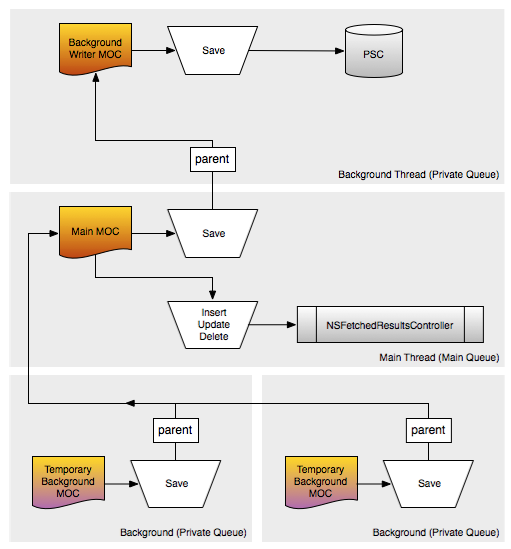
\includegraphics[scale=0.55]{img/coredataarch.png}
\caption{\label{fig:coredataarch}CoreData context architecture. Taken
  from~\cite{coredataarch}} 
\end{figure} 

The context attached to the persistent store saves all the data on disk, but on a
background thread, so the UI is never blocked. Then, all the save contexts that we
can create use a background thread and trigger the Main Thread, UI-context when they
have saved any info. This architecture is often known as \emph{child-context},
because there is a parent-child relationship between all the
contexts~\ref{fig:coredataarch}. 

\subsection{Augmented reality performance}
During the development of Ponster, both OpenCV and Vuforia have been tested. Due to
the low performance of OpenCV on mobile devices, Vuforia has been the chosen library
to bring the augmented reality to our app. In the [] chart we can find the average
time to perform each frame with the different technologies tested.



\section{Features}
The Ponster app has three main features: list posters, try how they look wherever
the user wants and capture an screenshot of the poster in the scene.

\begin{description}
\item [List posters] \hfill \\
\item [Augmented reality] \hfill \\
\item [Screenshot] \hfill \\
\end{description}
